\documentclass[11pt]{article}
\usepackage{fec}
\usepackage{mathtools}
\usepackage{longtable}
\usepackage{array}
\usepackage{graphicx}
\usepackage{lscape}
\usepackage{verbatim}
\usepackage{amsmath}
\usepackage{hhline}
\usepackage{subfigure}
\begin{document}
\title{Complexity of Pivot Algorithms}
\author{Qi Wang, Sean Kelley}
\date{December, 2020}
\maketitle


\begin{abstract}
Abstract...
\end{abstract}


\section{Introduction}
Simplex method was invented by Dantzig in 1947 \cite{dantzig1951maximization} to solve the Linear Optimization (LP) problem. It was tableau pivoting based method and pivoting under certain rules. The rules can be flexible so many simplex variants have been developed afterwards. Another framework of pivot algorithm is criss-cross method, which was proposed by Zionts at 1969 \cite{fukuda1997criss} and then \cite{terlaky1987finite}, \cite{chang1979least} present finite criss-cross version independently around 1980s. Some variant pivot methods appeared by proposing different pivots rules. We will describe them in the following section. \textbf{Mention Short simplex paths}\\
Although simplex method was generally efficient in practical, theoretically, Klee and Minty \cite{wikipediacontributors_2020_kleeminty} in 1970s showed the worst case that, a specific type of LO problem, a variant of simplex method visited all vertices (exponential steps) until solve the problem to be optimal. The feasible region of such problems was call Klee-Minty cube whose corners have been "squashed". We will demonstrate some examples in the following section. For now, it is still an unaccomplished problem that to design a pivot algorithm and prove that the number of pivot steps is bounded by polynomial of number of variables and constraints.
The paper is structured as follows: in Section 2 we define the LO problem, list the notation and (\textbf{might present some algorithms}); in section 3 we discuss the complexity of pivot algorithms and give a brief conclusion in the final section.

\section{The pivot algorithm for LO}
In this paper, we consider the Linear optimization problem of the standard form
\begin{align}
\begin{split}
\min \quad &c^Tx\\
\text{s.t.} \quad &Ax = b\\
&x \ge 0\\
 x \in \Rmbb^n,\ c \in \Rmbb^n,\ &A \in \Rmbb^{m\times n},\ b \in \Rmbb^m   
\end{split}
\end{align}
\begin{table}[h]
\caption{Notation}
\centering
\begin{tabular}{lll}
\hline
$n$ & number of variables   &  \\
$m$ & number of constraints (assume $m \le n$) &  \\
\hline
\end{tabular}
\end{table}
\section{Complexity - worst case}
Given $m$ constraints and $n$ variables, there are at most $\binom{n}{m}$ possible basis, which is the biggest upper bound for the number of iterations for pivot algorithms. When $m=\frac{n}{2}$, $\binom{n}{m}$ get its maximum $\binom{n}{\frac{n}{2}}\approx \sqrt{\frac{2}{\pi n}}2^n$. Klee and Minty defined a type of LO problems which some pivot algorithms may visit all vertices before finally finding the optimal solution. Detailed introduction of Klee Minty cube can be referred to \cite{vanderbei2020linear}. Here we demonstrate some examples. Klee Minty cube is defined as following LO problem \ref{eq:klLO}. The coefficients might be different in different articles. 
\begin{align}
\begin{split}
\max &\sum_{j=1}^n 2^{n-j}x_j \\
\text{s.t. } & 2\sum_{j=1}^{i-1}2^{i-j}x_j + x_i \le 5^i, \quad i=1,\cdots,n\\
			&x_j \ge 0,  \quad j=1,\cdots,n
\end{split}\label{eq:klLO}
\end{align} 
When $n=2$ and $n=3$ the 2-d and 3-d Klee Minty LO problems are 
\begin{align*}
\begin{split}
\max \quad & 2x_1 + x_2 \\
\text{s.t. }\quad  & x_1 \le 5\\
& 4x_1 + x_2 \le 25\\
& x_1 \ge 0,\ x_2 \ge 0.
\end{split}
\begin{split}
\max \quad & 4x_1 + 2x_2 + x_3 \\
\text{s.t. }\quad  & x_1 \le 5\\
& 4x_1 + x_2 \le 25\\
& 8x_1 + 4x_2 + x_3 \le 125\\
& x_1 \ge 0,\ x_2 \ge 0, \ x_3 \ge 0.
\end{split}
\end{align*}
The feasible region of 2-d and 3-d Klee Minty problems are shown in Figure \ref{fig:kmcube}. They look like "squashed" square and cube, which are very ill-conditioned.
\begin{figure}
    \centering
    \subfigure[]{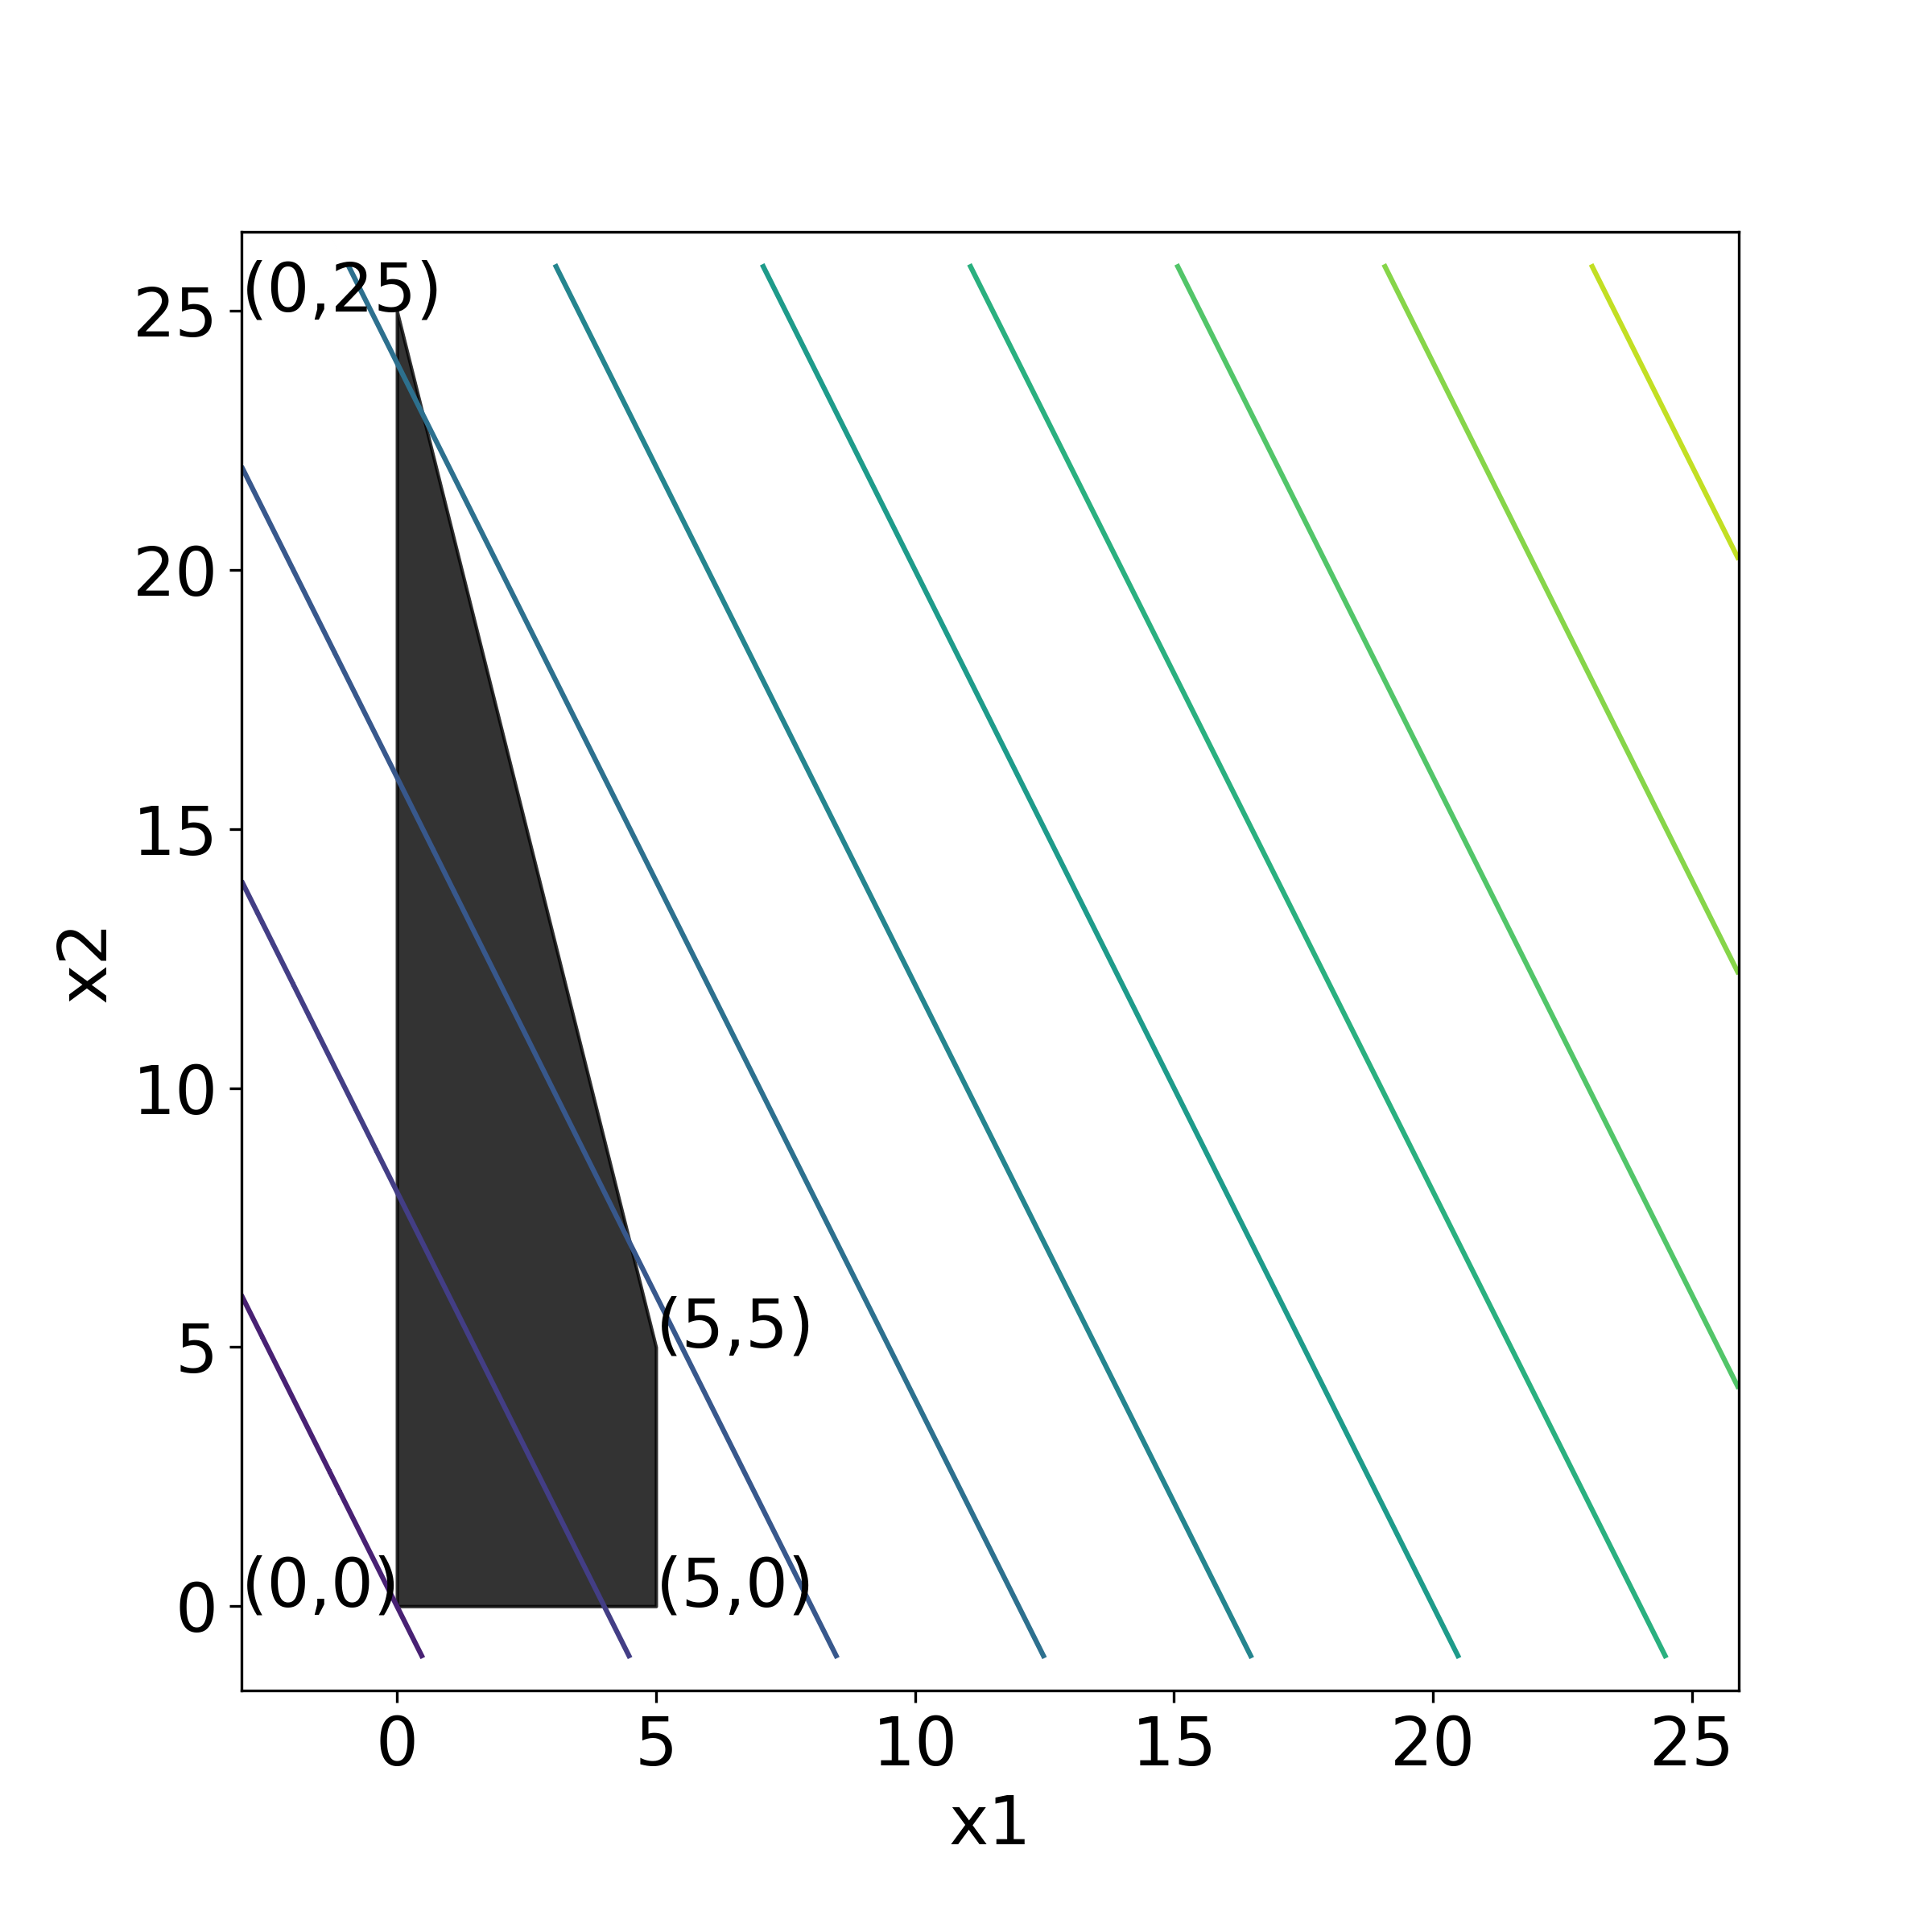
\includegraphics[width=0.38\textwidth]{klee_cube_d2.png}}
    \subfigure[]{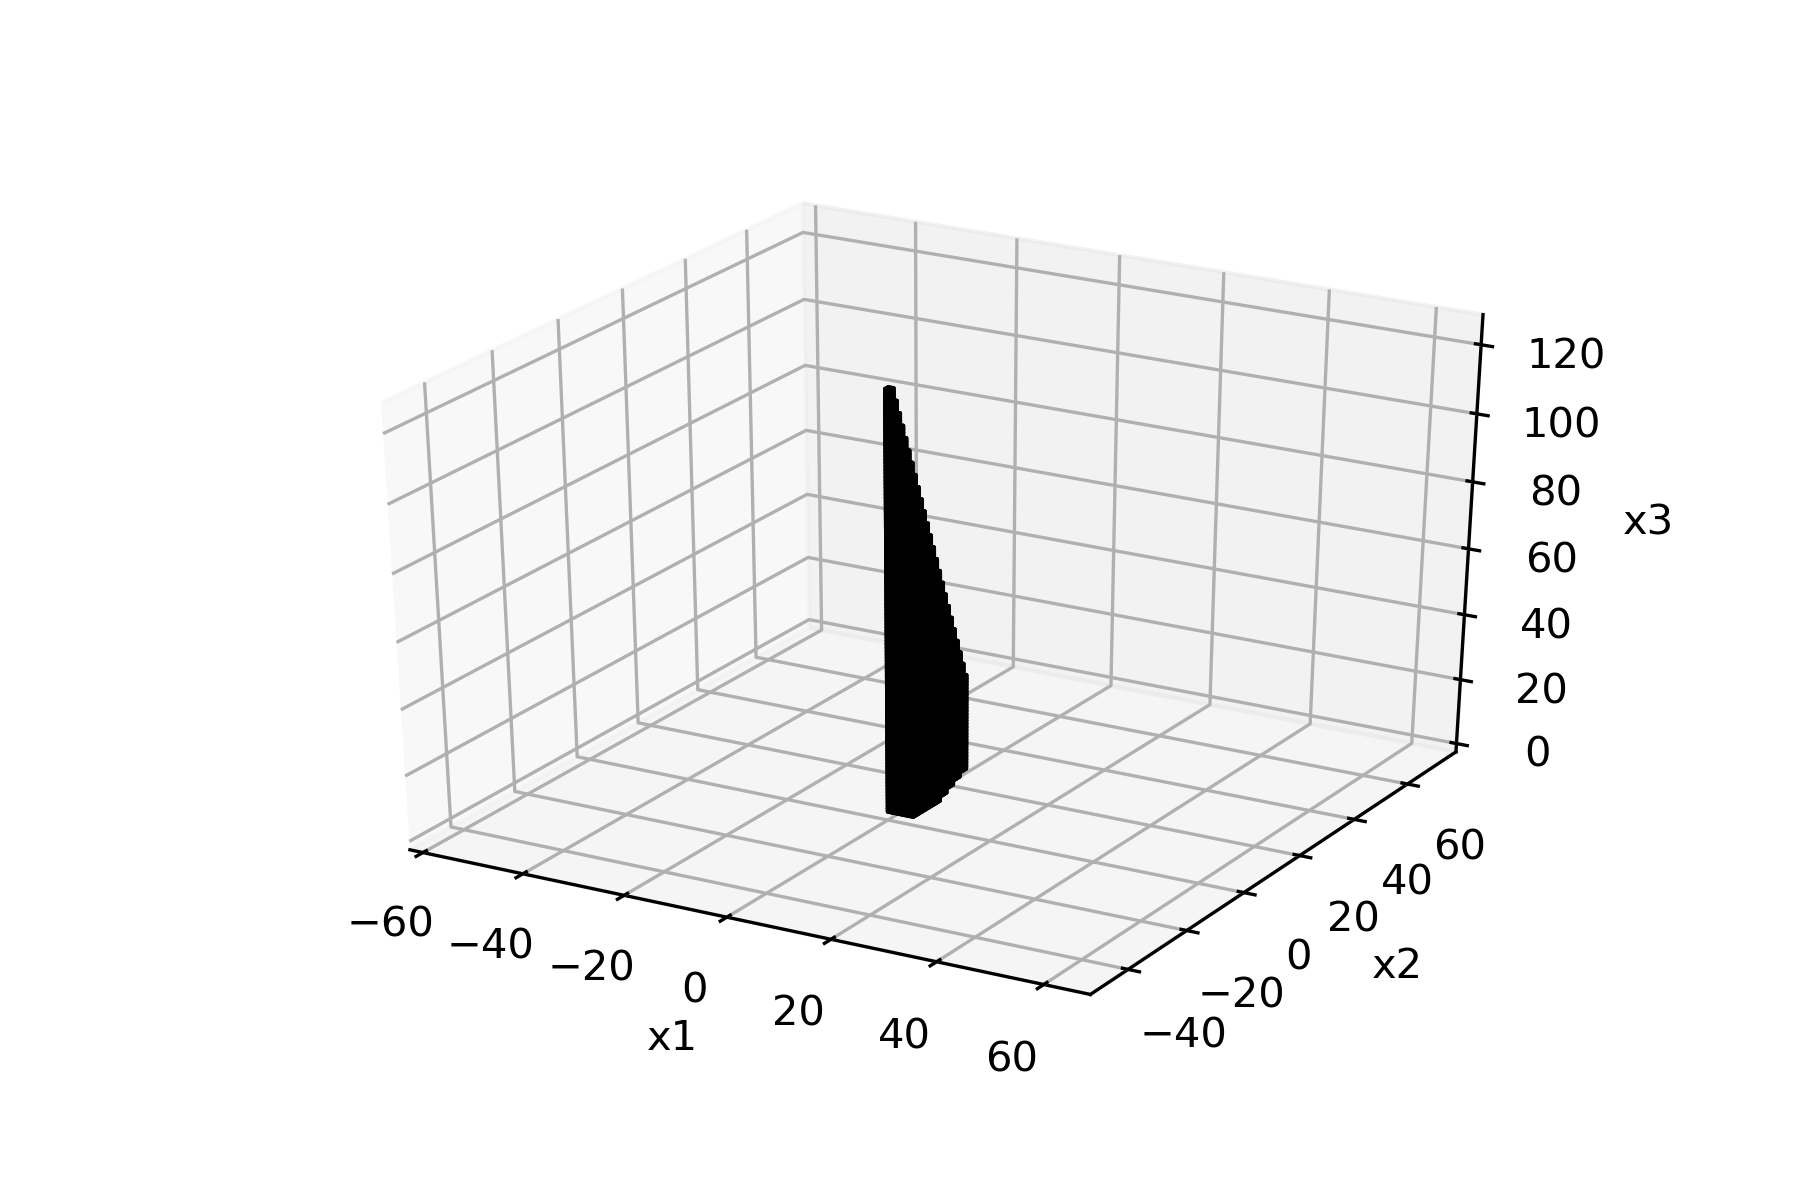
\includegraphics[width=0.59\textwidth]{klee_cube_d3.png}}
    \caption{(a) Feasible region of 2-d Klee Minty Cube with contour lines (b) Feasible region of 3-d Klee Minty Cube}
    \label{fig:kmcube}
\end{figure}
We apply primal simplex method (a) least-index version and (b) Dantzig (the nonbasis with biggest reduced cost enters) pivot rules to demonstrate the number of pivot steps. The tableau result of least-index pivot rule is shown in Table \ref{Table: tableau}. Note the results of Dantzig pivot rule and least-index rule coincide because in first iteration, the nonbasis with the most negative reduced cost is $x_1$ which is the entering nonbasis by least-index rule, too. 

\begin{table}[H]
\caption{Tableau of primal simplex method (least index version), the element with * is the pivot element. }
\label{Table: tableau}
\centering
\begin{tabular}{c|llllll}
   & rhs & $x_1$ & $x_2$ & $s_1$ & $s_2$ &                 \\ \cline{1-6}
$z$  & 0   & 2  & 1  & 0  & 0  & at vetex (0,0)  \\
$s_1$ & 5   & $1^*$  & 0  & 1  & 0  &                 \\
$s_2$ & 25  & 4  & 1  & 0  & 1  &                 \\ \hhline{======}
$z$  & -10 & 0  & 1  & -2 & 0  & at vetex (5,0)  \\
$x_1$ & 5   & 1  & 0  & 1  & 0  &                 \\
$s_2$ & 5   & 0  & $1^*$  & -4 & 1  &                 \\ \hhline{======}
$z$  & -15 & 0  & 0  & 2  & -1 & at vetex (5,5)  \\
$x_1$ & 5   & 1  & 0  & $1^*$  & 0  &                 \\
$x_2$ & 5   & 0  & 1  & -4 & 1  &                 \\ \hhline{======}
$z$  & -25 & -2 & 0  & 0  & -1 & at vetex (0,25) \\
$s_1$ & 5   & 1  & 0  & 1  & 0  &                 \\
$x_2$ & 25  & 4  & 1  & 0  & 1  &                 \\ \hhline{======}
\end{tabular}
\end{table}


%\section{title}
%There are certain pivot rules:
%\begin{itemize}
%\item Bland's rule, lexicographic rule
%\item Clairvoyant pivot rule (only theoretical), unimplementable
%\item Hirsch conjecture : disproven by Francisco Santos, 2011
%\item Polynomial Hirsch conjecture -- still open
%\end{itemize}


\section{Conclusion}
Conclusion...

\bibliographystyle{plain}
\bibliography{reference.bib} 

\section{Outline Suggestion}
what are pivot algorithms?
include point that there are two parts - selecting the pivot and making the pivot

Why did pivot algorithms come about?

what kinds are there?
simplex
criss cross

who developed them? when?

how do they differ (include problem assumptions/set up and iteration differences)?

what were their pivot calculation (everything) and pivot choosing rules (e.g. dantzigs rule - just most negative reduced cost/element in objective row)

what were their complexity?
O(something) when nondegenerate in worst case
degeneracy could still create infiniteness/nonconvergence

what is degeneracy?

why does degeneracy matter (how does it affect complexity)?

how did we get around degeneracy?
zadeh's/cunningham's rules
blands rule

What did this bring complexity to?
same as before, now just covering a much wider array of problems
now all were finite/convergent

How could we improve this?
either improve the pivot operation or the pivot selection

How could we improve the pivot operations?
Revised simplex method

What is the revised simplex method? Who worked on this and when?

What did this bring complexity to?

This became the basis for modern solvers using pivot algorithms (get confirmed by gurobi/cplex/xpress/coin)
mention improvements made by preprocessing, but don't go into detail - not sure if they are problem specific or general to pivot algorithms

Why worry about improving pivot selection?
pivot algorithms usually average polynomial time complexity
but klee-minty showed that worst case complexity can actually be achieved
(what is klee-minty)

What were some early "improvements" to pivot selection?
Greatest Improvement (calculates which column reduces objective the most)
Steepest edge (normalize reduced cost with the norm of its column)
(I think these were actually slower in the average case because when you have a lot of variables the quick calculations on bland's rule win out)

Ok this is where I am stuck - these things cover us nicely until 1980's and our papers pick up 2010's. I feel like we should have something to fit the in between in terms of advancement of computational complexity of pivot algorithms


\end{document}
